%##################################################################################################

The tasks within the \texttt{build} category of our benchmark are devised to evaluate an AI agent's aptitude in structural reasoning, spatial organization, and its capability to interact with and manipulate the environment to create specific structures or outcomes. Building is an integral component of Minecraft gameplay, requiring an intricate interplay of planning, creativity, and understanding of block properties. 

\begin{figure*}[h]
%\framebox[4.0in]{$\;$}
\begin{center}
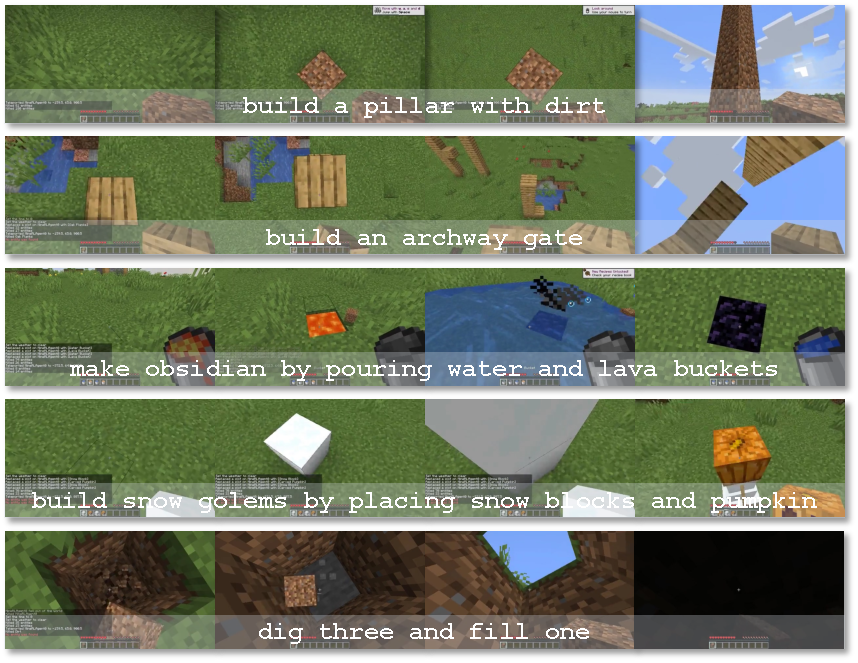
\includegraphics[scale = 0.9]{figures/benchmark_build.pdf}
\end{center}
\caption{Examples of tasks in \texttt{build} category. }
\end{figure*}

\definecolor{codeblue}{rgb}{0.25,0.5,0.5}
\definecolor{codekw}{rgb}{0.85, 0.18, 0.50}
\definecolor{keywordgreen}{rgb}{0,0.6,0}
\lstset{
  backgroundcolor=\color{gray!10},
  basicstyle=\fontsize{8pt}{9pt}\ttfamily\selectfont,
  columns=fullflexible,
  breaklines=true,
  captionpos=b,
  commentstyle=\fontsize{7.5pt}{7.5pt}\color{codeblue},
  keywords = {Task, Description, Time, Evaluation, Precondition, SkillAssessed}, 
  keywordstyle = {\textbf},
  caption={The environment configuration and evaluation metric for \texttt{build} series tasks. },
  label={lst:minecraft_deps_prompt}
}
\begin{lstlisting} % [language=python]  

Task: build pillar
Description: Build a pillar with dirt. 
Precondition: Spawn the player in the plains biome with a stack of dirt in the main hand. 
SkillAssessed: Vertical construction and basic structure formation.
Evaluation: Just run away. < Look down. < Jump and place the dirt. < Pile the dirt into a few pillars. < Make a really high pillar.

Task: dig three down and fill one up
Description: Dig three dirt blocks and fill the hole above.  
Precondition: Spawn the player in the plains biome. 
SkillAssessed: Ground manipulation and depth perception. 
Evaluation: Just run away. < Look down. < Dig down three dirt blocks. < Raise the head. < Raise the head and use dirt to fill the hole. 

Task: build gate
Description: Build an archway gate. 
Precondition: Spawn the player in the plains biome with a stack of oak_planks in the main hand. 
SkillAssessed: Symmetry, planning, and aesthetic construction.
Evaluation: Place no plank. < Build 1 pillar. < Build 2 pillars. < Build an archway gate. 

Task: build obsidian
Description: Make obsidian by pouring a water bucket and a lava bucket. 
Precondition: Spawn the player in the plains biome with two water buckets and two lava buckets in the Hotbar. 
SkillAssessed: Material transformation, understanding of in-game chemistry, and precise pouring.
Evaluation: Just run away. < Pour water or lava. < Pour both liquids. < Pour into a mold to make obsidian. 

Task: build snow golems
Description: Build snow golems by placing two snow blocks and one carved pumpkin. 
Precondition: Spawn the player in the plains biome with two stacks of snow blocks and two stacks of carved pumpkins in the Hotbar. 
SkillAssessed: Entity creation, sequential block placement, and combination of multiple materials. 
Evaluation: Place no block. < Place at least one kind of block. < Place both kinds of blocks. < Build a snow golem. 

\end{lstlisting}


